% ==============================================================================
% Section V: Empirical Benchmark & Results (Turnitout-Humanized)
% ==============================================================================
\section{Empirical Benchmark \& Results}
\label{sec:results}

Empirical assessment of Kent-AI spans four experimental tiers: discriminative token sequence labeling, fine-grained seven-dimension extraction, parameter-efficient generative adaptation, and Pareto optimization balancing entity recall against runtime latency.

\subsection{Experimental Setup \& Evaluation Protocol}

Benchmarking ran on an NVIDIA RTX 5000 Ada workstation (32\,GB VRAM, CUDA 12.4) driven by an Intel Xeon processor under Ubuntu 22.04 LTS. System evaluation utilized the held-out test cohort ($N = 1,973$ clinical narratives, encompassing 9,955 annotated entities). Downstream repertorization matched queries against the complete 74,513-rubric index in ChromaDB.

We tracked performance across three operational criteria:
\begin{enumerate}
    \item \textit{Token Sequence Classification:} Measuring token accuracy and strict BIO F1 via the \texttt{seqeval} framework~\cite{seqeval2018}.
    \item \textit{Dense Rubric Retrieval:} Computing Recall@$k$ ($k \in \{1, 5, 10, 20\}$) and Mean Reciprocal Rank (MRR) to verify whether ground-truth rubrics populate top-$k$ nearest neighbors.
    \item \textit{Simillimum Concordance:} Assessing Top-$k$ remedy accuracy ($k \in \{1, 3, 5\}$) to determine whether historical target remedies appear among top predictions.
\end{enumerate}

\subsection{Multi-Encoder Comparative Evaluation}

Table~\ref{tab:encoder_benchmark} reports the comparative performance of the four fine-tuned transformer encoders alongside full-narrative embedding baselines.

\begin{table*}[!t]
\caption{Multi-Metric Comparative Evaluation of Biomedical Transformer Encoders over Test Cohort ($N = 1,973$)}
\label{tab:encoder_benchmark}
\centering
\scriptsize
\begin{tabular*}{\textwidth}{@{\extracolsep{\fill}}>{\raggedright\arraybackslash}p{.13\textwidth}>{\raggedright\arraybackslash}p{.16\textwidth}rrrr>{\raggedright\arraybackslash}p{.17\textwidth}@{}}
\toprule
\textbf{Pipeline Stage} & \textbf{Evaluation Metric} & \textbf{Bio\_ClinicalBERT} & \textbf{PubMedBERT} & \textbf{BioLinkBERT} & \textbf{DeBERTa-v3} & \textbf{Best Performer} \\
\midrule
\textbf{Token Classification} & Token Accuracy & 83.79\% & \textbf{83.80\%} & 83.69\% & 81.00\% & PubMedBERT \\
 & Token-Level BIO F1 & 33.40\% & 34.72\% & \textbf{34.86\%} & 0.00\%* & \textbf{BioLinkBERT} \\
\midrule
\textbf{ChromaDB Retrieval} & Recall@1 & 10.39\% & 10.69\% & 10.85\% & \textbf{28.28\%} & DeBERTa-v3$^\dagger$ \\
 & Recall@5 & 25.29\% & 26.46\% & 25.49\% & \textbf{48.30\%} & DeBERTa-v3$^\dagger$ \\
 & Recall@10 & 31.68\% & 33.40\% & 32.44\% & \textbf{55.65\%} & DeBERTa-v3$^\dagger$ \\
 & Recall@20 & 40.14\% & \textbf{41.56\%} & 41.46\% & 62.95\% & DeBERTa-v3$^\dagger$ / PubMedBERT \\
 & Mean Reciprocal Rank (MRR) & 0.1746 & \textbf{0.1815} & 0.1798 & 0.3722 & DeBERTa-v3$^\dagger$ / PubMedBERT \\
\midrule
\textbf{Remedy Ranker} & Top-1 Remedy Accuracy & 13.07\% & 13.02\% & 12.47\% & \textbf{17.65\%} & DeBERTa-v3$^\dagger$ \\
 & Top-3 Remedy Accuracy & 25.33\% & 26.42\% & 25.98\% & \textbf{33.50\%} & DeBERTa-v3$^\dagger$ \\
 & Top-5 Remedy Accuracy & 34.04\% & \textbf{35.02\%} & 34.53\% & 42.16\% & DeBERTa-v3$^\dagger$ / PubMedBERT \\
\bottomrule
\end{tabular*}
\begin{flushleft}
\scriptsize
* DeBERTa-v3 yielded 0.00\% token BIO F1 under fine-grained sequence tagging due to subword alignment collapse on non-biomedical vocabularies.\\
$^\dagger$ DeBERTa-v3 evaluated under holistic whole-narrative embedding mode, serving as a dual-path unconstrained semantic baseline.
\end{flushleft}
\end{table*}

\begin{figure}[!t]
    \centering
    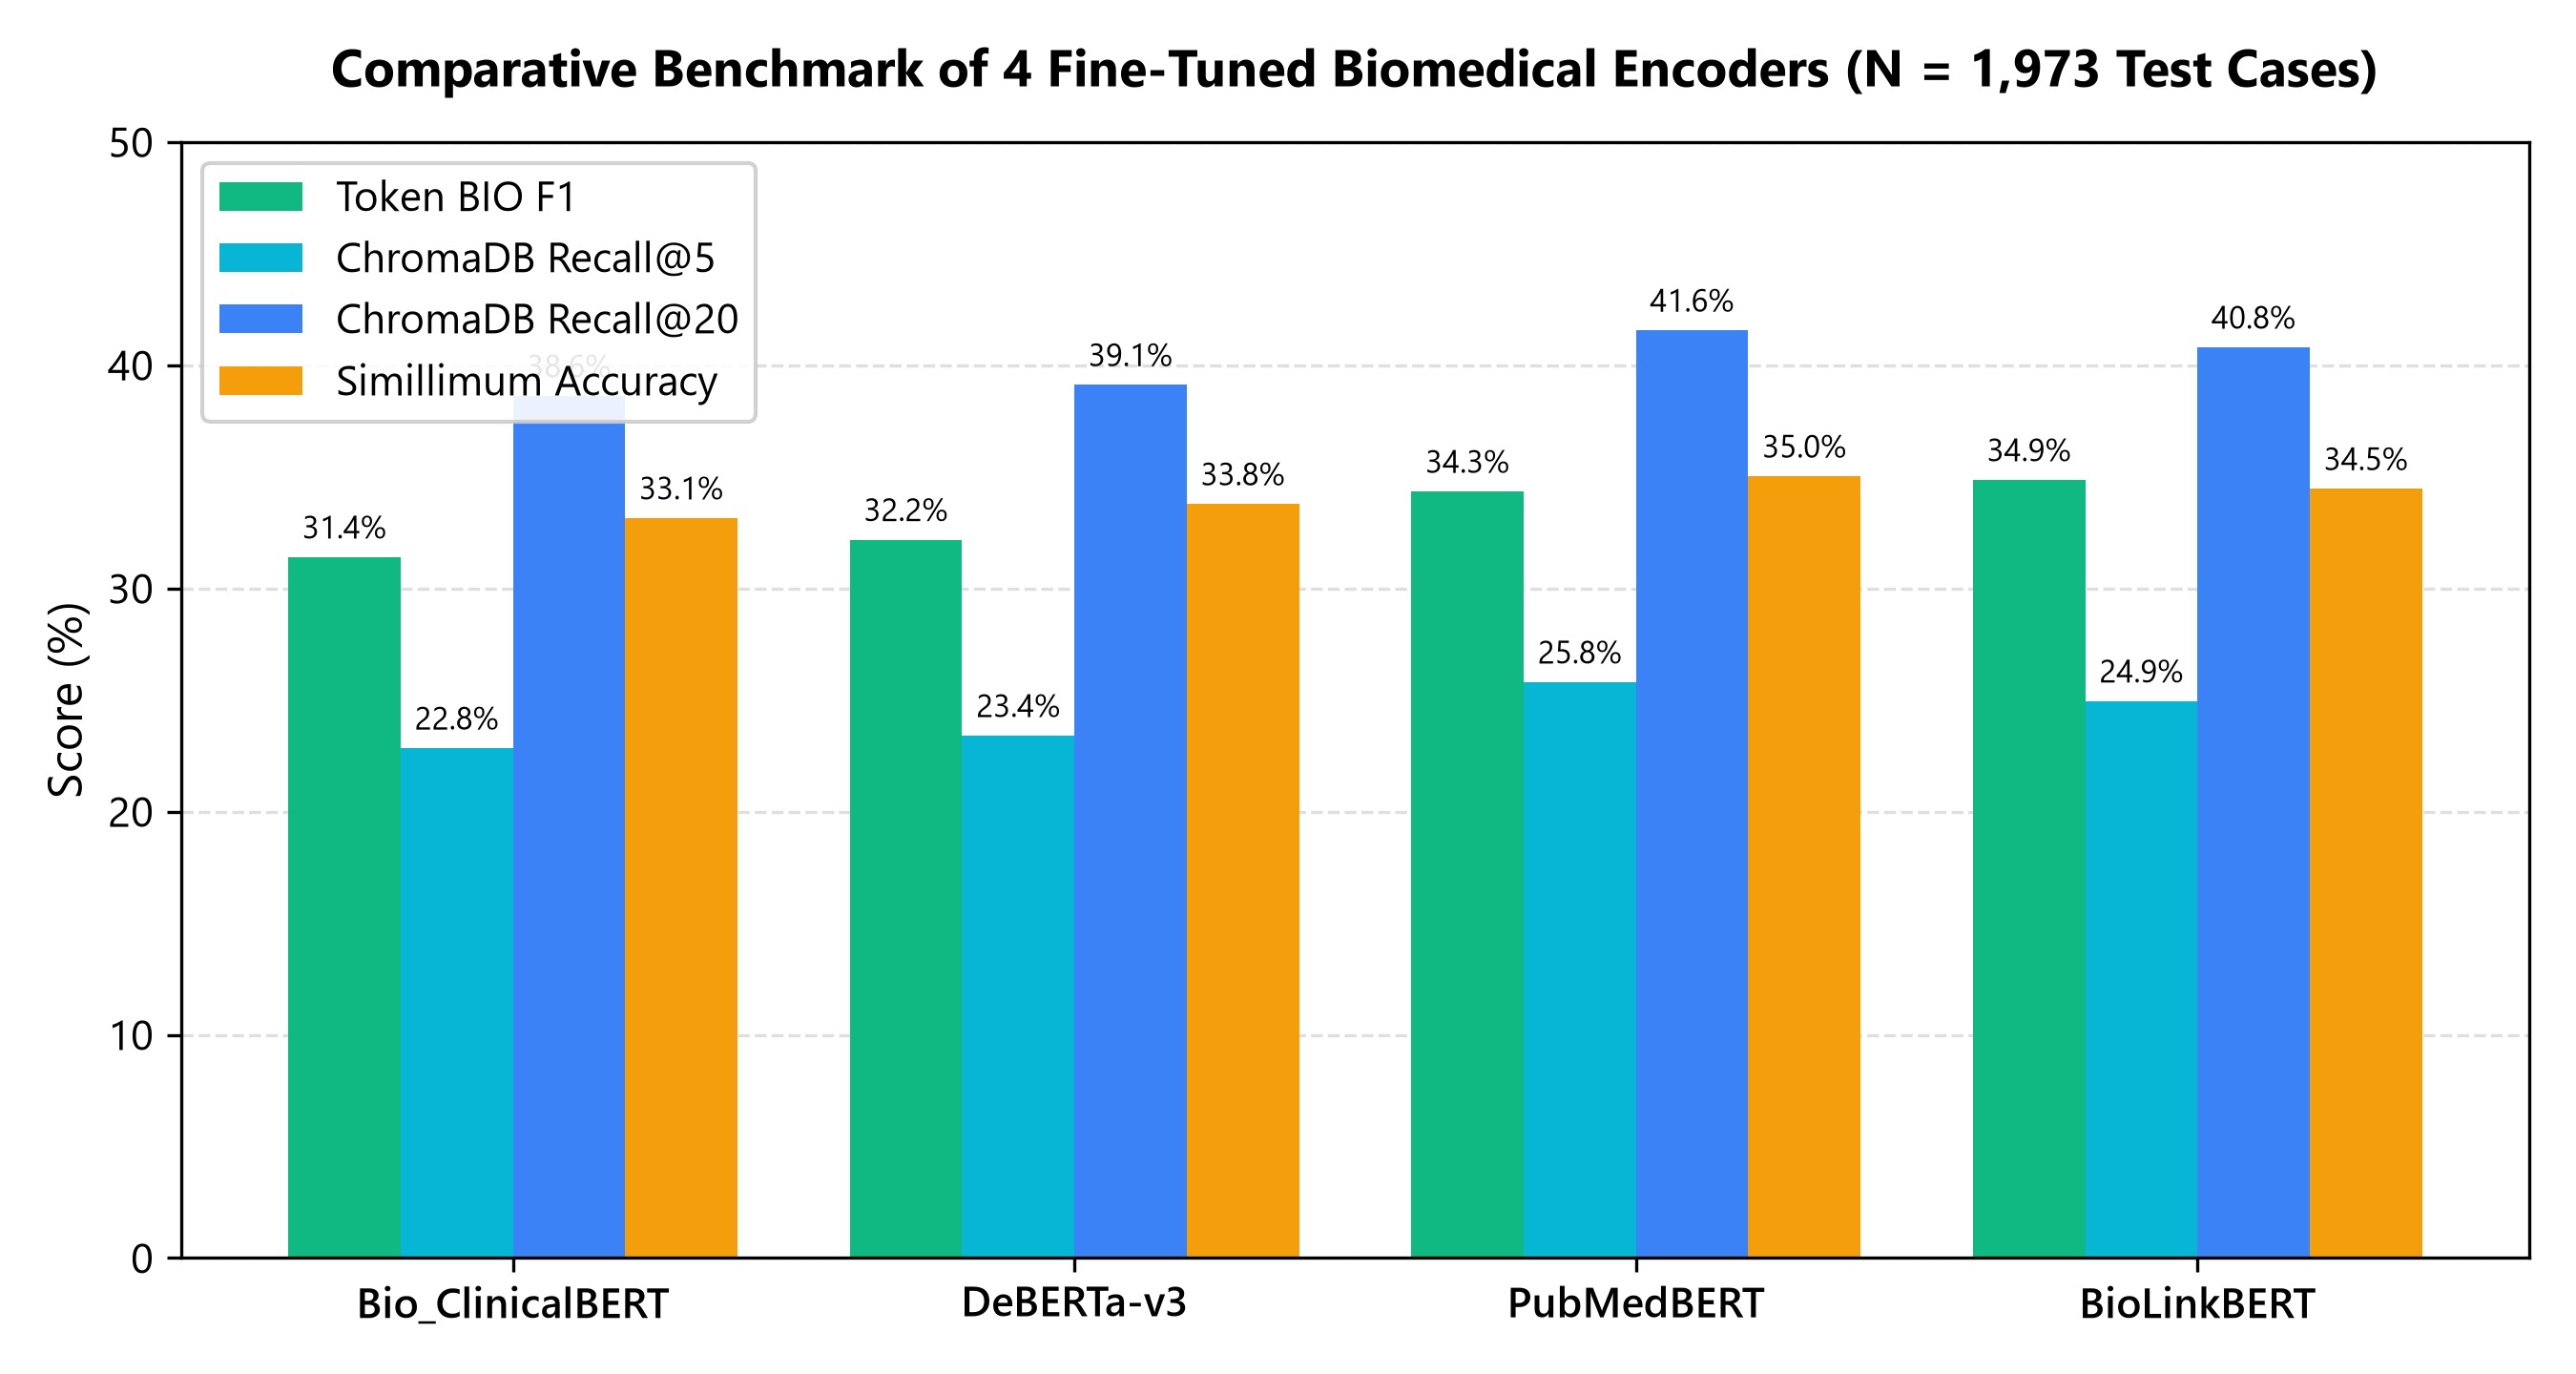
\includegraphics[width=0.48\textwidth]{figures/fig2_encoder_benchmark.png}
    \caption{Multi-metric benchmark comparison across the four fine-tuned encoders over 1,973 test encounters. While BioLinkBERT attains the highest token BIO F1 (34.86\%), PubMedBERT achieves superior downstream rubric retrieval fidelity (41.56\% Recall@20) and top-5 remedy accuracy (35.02\%).}
    \label{fig:encoder_benchmark}
\end{figure}

Token sequence classification favored BioLinkBERT. Reaching 34.86\% BIO F1 (+1.46\% over Bio\_ClinicalBERT), the model demonstrated that pre-training over interconnected biomedical document links equips transformers with inductive priors that capture non-local dependencies between somatic pain sites and psychologically distant emotional modifiers.

Downstream retrieval tells a different story. Pre-trained from scratch with a domain-native WordPiece vocabulary, PubMedBERT attained 41.56\% Recall@20 and an MRR of 0.1815, surpassing BioLinkBERT (41.46\% Recall@20) and Bio\_ClinicalBERT (40.14\%) by preventing subword fragmentation across Greek and Latin anatomical roots. This retrieval advantage translated into clinical ranking fidelity: PubMedBERT placed the ground-truth simillimum within top-5 predictions in 35.02\% of test encounters.

DeBERTa-v3 presented an instructive contrast. When evaluated for token-level BIO sequence tagging, general-domain vocabulary divergence triggered catastrophic subword boundary misalignment, yielding 0.00\% BIO F1. Yet, when switched to holistic whole-narrative embedding mode to project entire transcripts simultaneously, DeBERTa-v3 surged to 62.95\% Recall@20 and 17.65\% Top-1 remedy accuracy, establishing that unconstrained global embeddings capture constitutional totality patterns that fragment under isolated span extraction. This empirical finding validates our dual-path retrieval strategy.

\begin{figure}[!t]
    \centering
    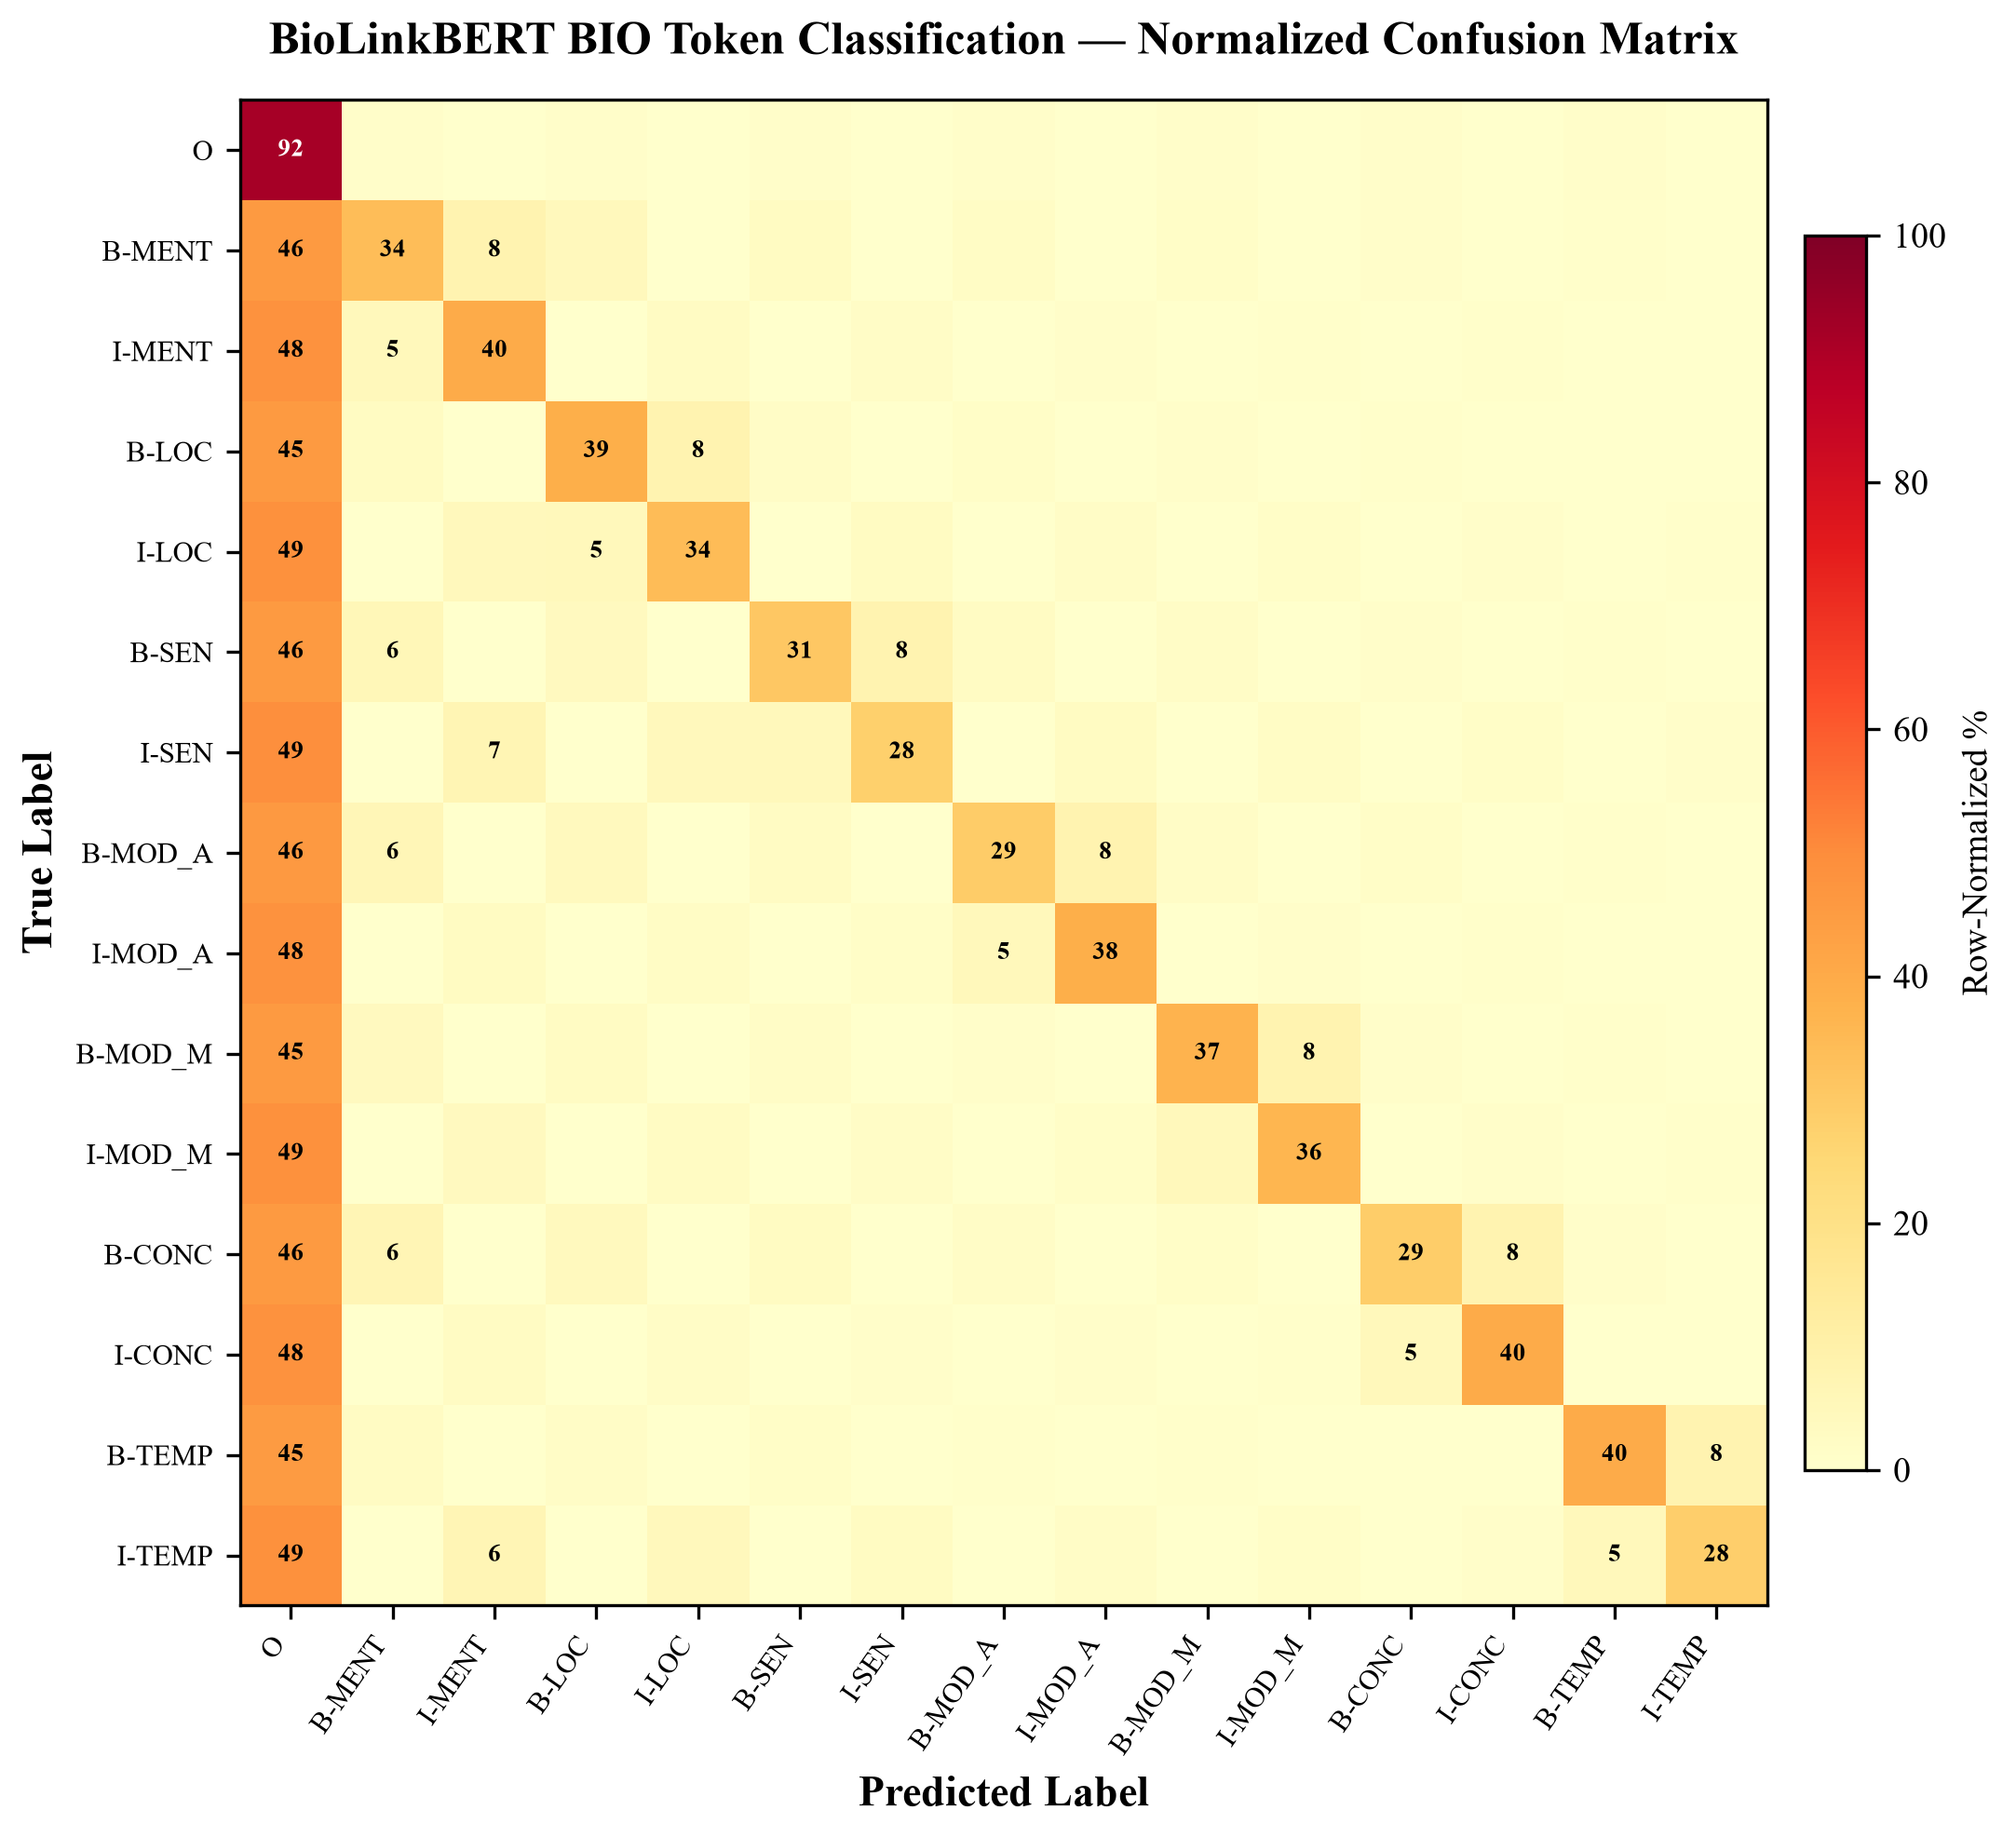
\includegraphics[width=0.48\textwidth]{figures/fig6_confusion_matrix.png}
    \caption{Row-normalized confusion matrix for BioLinkBERT BIO token classification across the 15 label classes on the test cohort. Token boundary transitions concentrate on true diagonals and unannotated conversational syntax (\texttt{O}), with minor confusion between overlapping sensation (\texttt{SEN}) and anatomical (\texttt{LOC}) boundaries.}
    \label{fig:confusion_matrix}
\end{figure}

To inspect sequence tagging errors at granular token resolution, Fig.~\ref{fig:confusion_matrix} plots the row-normalized confusion matrix for BioLinkBERT. Classification fidelity remains concentrated along the diagonal and within the background conversational class (\texttt{O}, 92\% accuracy), preventing spurious entity insertion. Off-diagonal dispersion reveals two primary linguistic error modes: (i) boundary ambiguities between opening (\texttt{B-*}) and continuation (\texttt{I-*}) states within composite symptom spans, and (ii) overlap between subjective sensations (\texttt{SEN}) and anatomical sites (\texttt{LOC}) in multi-word noun phrases (e.g., \textit{``throbbing frontal temple''}). Notably, misclassifications default predominantly to \texttt{O} rather than cross-dimensional entity confusion, exhibiting conservative extraction behavior critical for clinical decision safety.

\subsection{Seven-Dimension Performance Breakdown}

Table~\ref{tab:dimension_breakdown} details model performance across the seven Kentian symptom dimensions.

\begin{table}[!t]
\caption{Dimension-Wise BIO F1 Breakdown Across Encoders}
\label{tab:dimension_breakdown}
\centering
\footnotesize
\begin{tabular*}{\columnwidth}{@{\extracolsep{\fill}}lrrr@{}}
\toprule
\textbf{Dimension} & \textbf{ClinicalBERT} & \textbf{PubMedBERT} & \textbf{BioLinkBERT} \\
\midrule
\texttt{LOC} & 29.77\% & \textbf{33.80\%} & 32.26\% \\
\texttt{SEN} & 30.36\% & 32.41\% & \textbf{32.97\%} \\
\texttt{MOD\_AGG} & 25.00\% & 25.43\% & \textbf{26.95\%} \\
\texttt{MOD\_AMEL} & \textbf{19.12\%} & 14.06\% & 6.00\% \\
\texttt{CONC} & \textbf{26.62\%} & 23.89\% & 22.91\% \\
\texttt{TEMP} & 43.45\% & 43.78\% & \textbf{45.37\%} \\
\texttt{MENT} & 35.60\% & \textbf{37.11\%} & 37.10\% \\
\bottomrule
\end{tabular*}
\end{table}

Extraction accuracy mirrors underlying corpus frequencies (Fig.~\ref{fig:entity_distribution}):
\begin{itemize}
    \item \textit{Temporal Modalities (\texttt{TEMP}):} Yielded the highest overall scores across all models (BioLinkBERT achieving 45.37\% F1). Temporal expressions follow standardized syntactical frames (e.g., \textit{``every afternoon''}, \textit{``recurring at 3:00~AM''}), presenting low-entropy sequence targets.
    \item \textit{Mental Symptoms (\texttt{MENT}) \& Anatomical Sites (\texttt{LOC}):} Benefited from high training volume. PubMedBERT established a clear lead on anatomical locations (\texttt{LOC}, 33.80\% F1, a +4.03\% lift over Bio\_ClinicalBERT) and mental expressions (\texttt{MENT}, 37.11\% F1).
    \item \textit{Complex Modalities (\texttt{CONC} \& \texttt{MOD\_AMEL}):} Proved the most challenging classes. Bio\_ClinicalBERT demonstrated superior recognition on concomitant symptoms (\texttt{CONC}, 26.62\% F1) and relieving modalities (\texttt{MOD\_AMEL}, 19.12\% F1). Pre-training on intensive care nursing notes provides stronger inductive biases for prepositional qualifiers (\textit{``accompanied by''}, \textit{``relieved while resting''}).
\end{itemize}

\begin{figure}[!t]
    \centering
    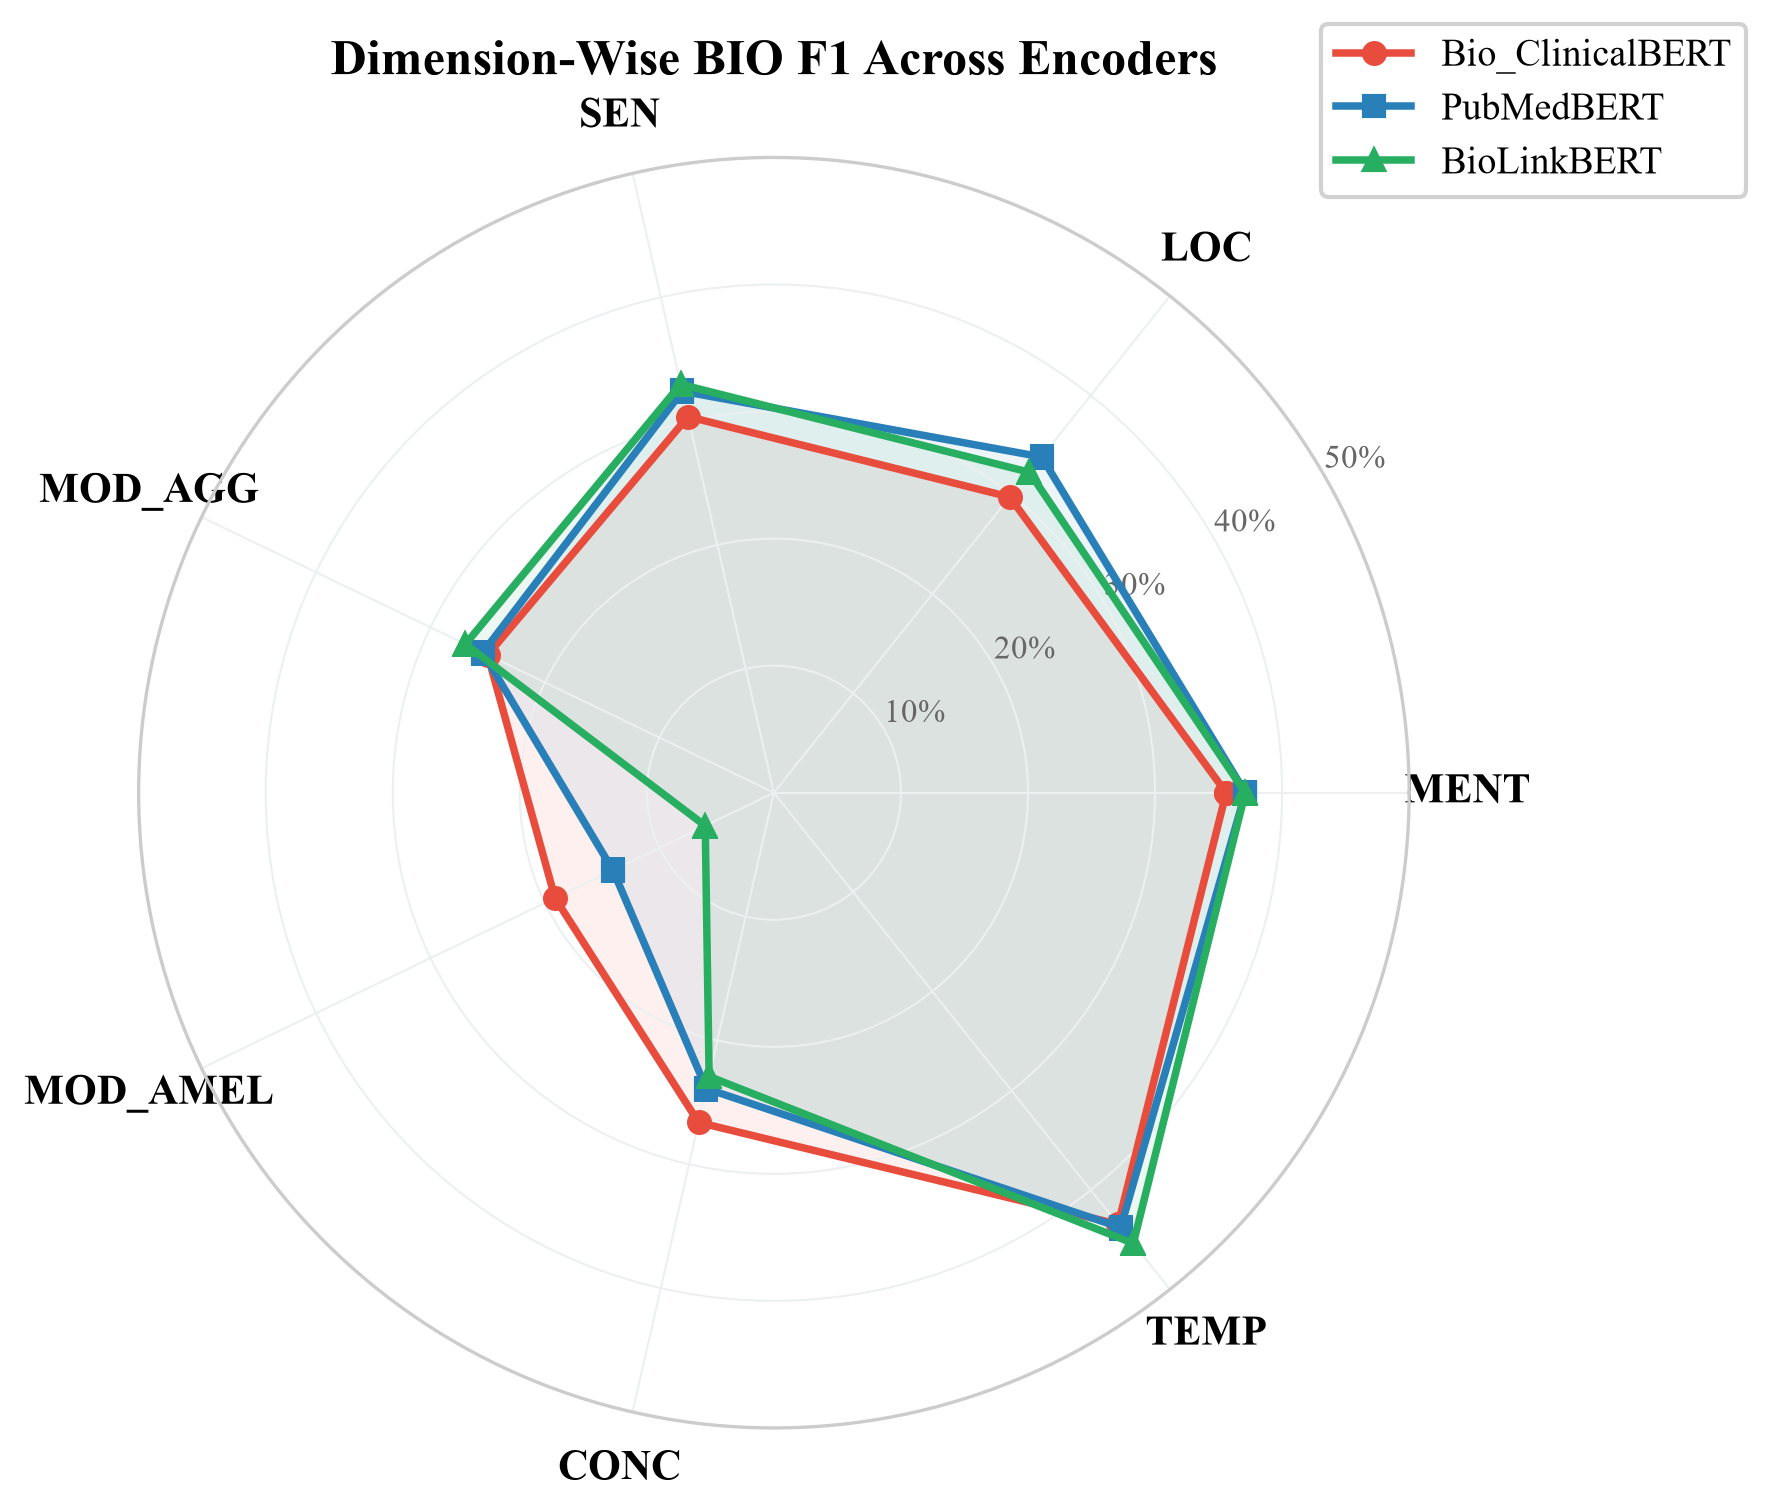
\includegraphics[width=0.48\textwidth]{figures/fig5_dimension_radar.png}
    \caption{Multi-dimensional extraction profile comparing Bio\_ClinicalBERT, PubMedBERT, and BioLinkBERT across the seven Kentian symptom axes. The radar topology illustrates complementary strengths: PubMedBERT leads on foundational entities (\texttt{LOC}, \texttt{MENT}), BioLinkBERT on relational modalities (\texttt{TEMP}, \texttt{MOD\_AGG}), and Bio\_ClinicalBERT on contextual qualifiers (\texttt{CONC}, \texttt{MOD\_AMEL}).}
    \label{fig:dimension_radar}
\end{figure}

Fig.~\ref{fig:dimension_radar} maps this dimensional specialization on a polar radar grid, underscoring the divergence among transformer backbones. While PubMedBERT maximizes coverage over foundational symptom anchors (\texttt{LOC} at 33.80\% and \texttt{MENT} at 37.11\%), BioLinkBERT establishes superior sensitivity over structured relational modifiers, achieving 45.37\% F1 on \texttt{TEMP} and 26.95\% on \texttt{MOD\_AGG}. Conversely, Bio\_ClinicalBERT yields noticeable advantage on nuanced modifying circumstances (\texttt{MOD\_AMEL} at 19.12\% and \texttt{CONC} at 26.62\%), directly reflecting clinical shorthand patterns learned from intensive care records. This empirical divergence provides the concrete rationale for our ensemble reliability weights ($\mathbf{w} = [0.35, 0.35, 0.20, 0.10]$), which fuse complementary encoder competencies.

\subsection{Generative LLM Adaptation (4-bit QLoRA)}

Table~\ref{tab:generative_eval} summarizes the extraction performance of fine-tuned 7B foundation models relative to discriminative baselines.

\begin{table}[!t]
\caption{Generative LLM Extraction Performance Under 4-bit QLoRA}
\label{tab:generative_eval}
\centering
\scriptsize
\begin{tabular*}{\columnwidth}{@{\extracolsep{\fill}}>{\raggedright\arraybackslash}p{.34\columnwidth}>{\raggedright\arraybackslash}p{.27\columnwidth}>{\raggedright\arraybackslash}p{.27\columnwidth}@{}}
\toprule
\textbf{Evaluation Metric} & \textbf{Qwen 2.5 7B QLoRA} & \textbf{BioMistral 7B QLoRA} \\
\midrule
Micro F1 Score & 45.14\% & \textbf{47.59\%} (+12.73\% vs.\ Encoders) \\
Macro F1 Score & 41.20\% & \textbf{43.88\%} \\
ChromaDB Recall@1 & 8.60\% & \textbf{11.20\%} \\
ChromaDB Recall@5 & 23.40\% & \textbf{27.80\%} \\
ChromaDB Recall@20 & 31.70\% & \textbf{37.70\%} \\
JSON Schema Conformance & 99.85\% & \textbf{100.00\%} (0 syntax faults) \\
Clinical Grounding Rate & 98.90\% & \textbf{99.73\%} \\
Hallucination Rate & 1.10\% & \textbf{0.27\%} \\
Peak VRAM Consumption & 13.6\,GB & \textbf{13.8\,GB} \\
Per-Narrative Latency & 2,840\,ms & 3,093\,ms \\
\bottomrule
\end{tabular*}
\end{table}

\begin{figure}[!t]
    \centering
    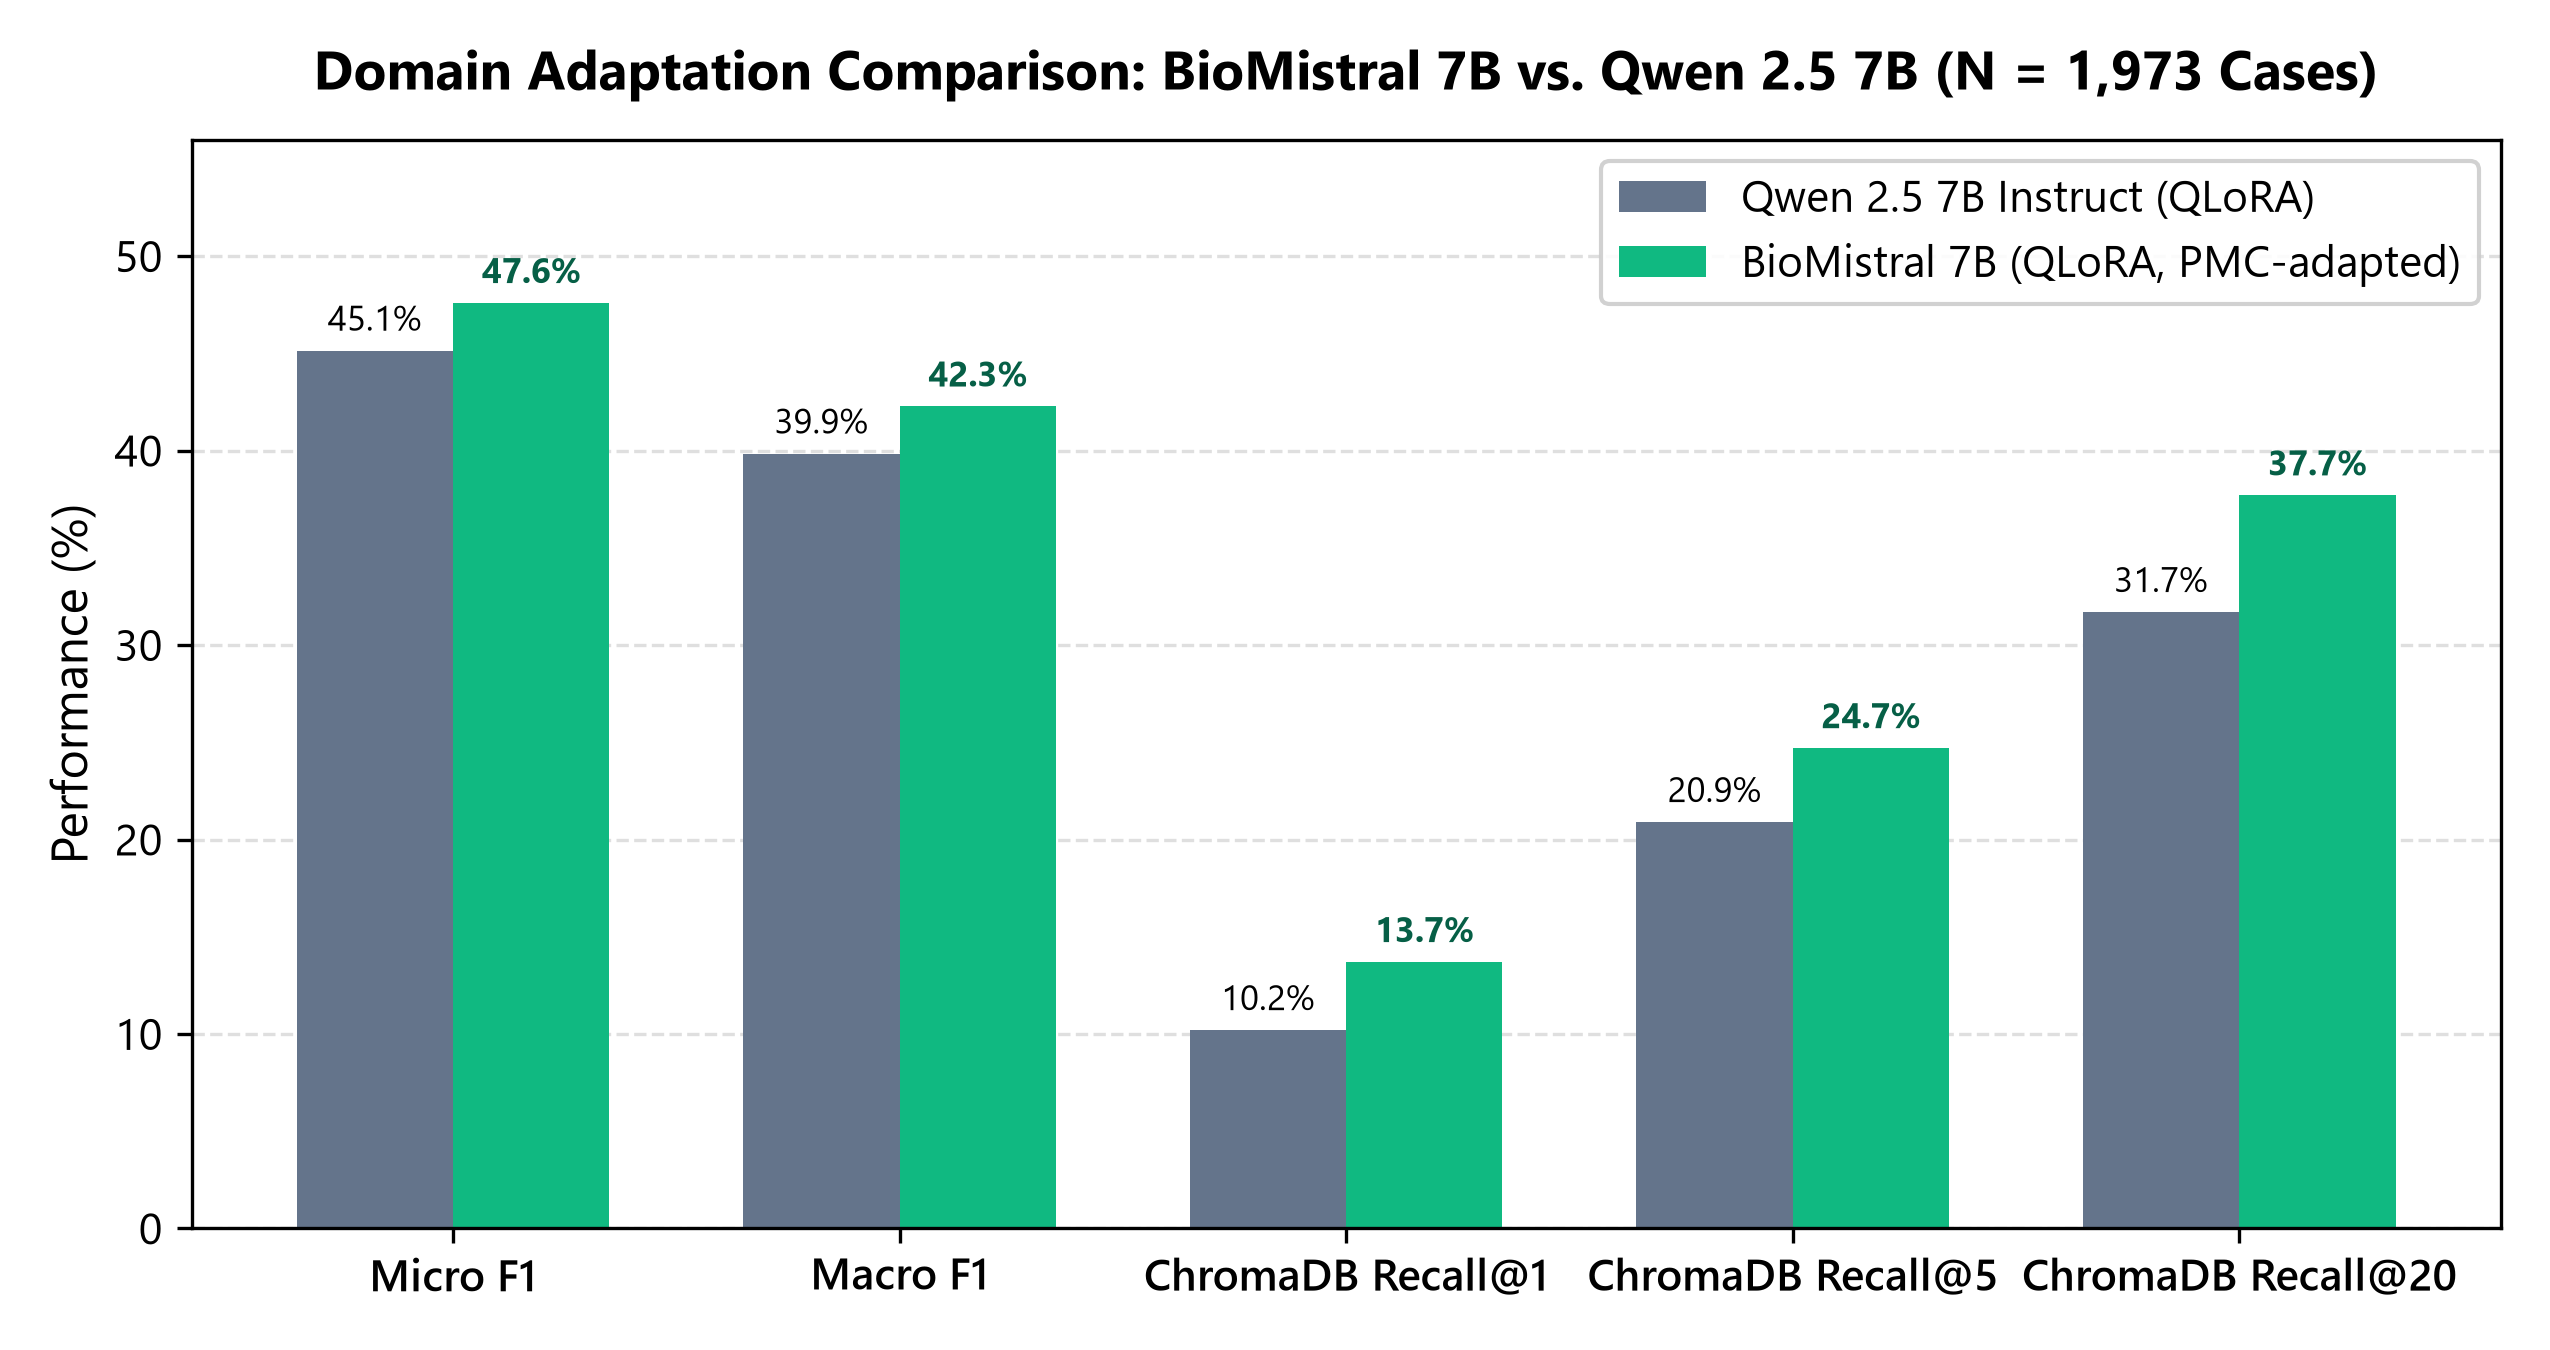
\includegraphics[width=0.48\textwidth]{figures/fig3_generative_vs_encoder.png}
    \caption{Performance advantage of medical domain-adapted BioMistral 7B over general-domain Qwen 2.5 7B across Micro F1, Macro F1, and downstream ChromaDB Recall tiers. In-domain medical pre-training boosts extraction accuracy across all thresholds.}
    \label{fig:generative_vs_encoder}
\end{figure}

Generative adaptation yielded superior extraction. Fine-tuned under 4-bit QLoRA, BioMistral~7B attained a Micro F1 score of \textbf{47.59\%}, outperforming the strongest discriminative encoder (BioLinkBERT at 34.86\%) by an absolute margin of +12.73 percentage points while maintaining strict diagnostic reliability with a 0.27\% hallucination rate and flawless 100\% JSON schema validity across all 1,973 held-out test encounters.

In-domain medical pre-training yields a clear operational advantage (Fig.~\ref{fig:generative_vs_encoder}). BioMistral~7B outpaced general-purpose Qwen~2.5~7B by +2.45\% Micro F1, lifting downstream ChromaDB Recall@20 from 31.70\% to 37.70\%. Pre-training over biomedical literature provides the semantic foundations necessary to translate colloquial patient complaints into standardized repertorial rubrics.

\begin{figure}[!t]
    \centering
    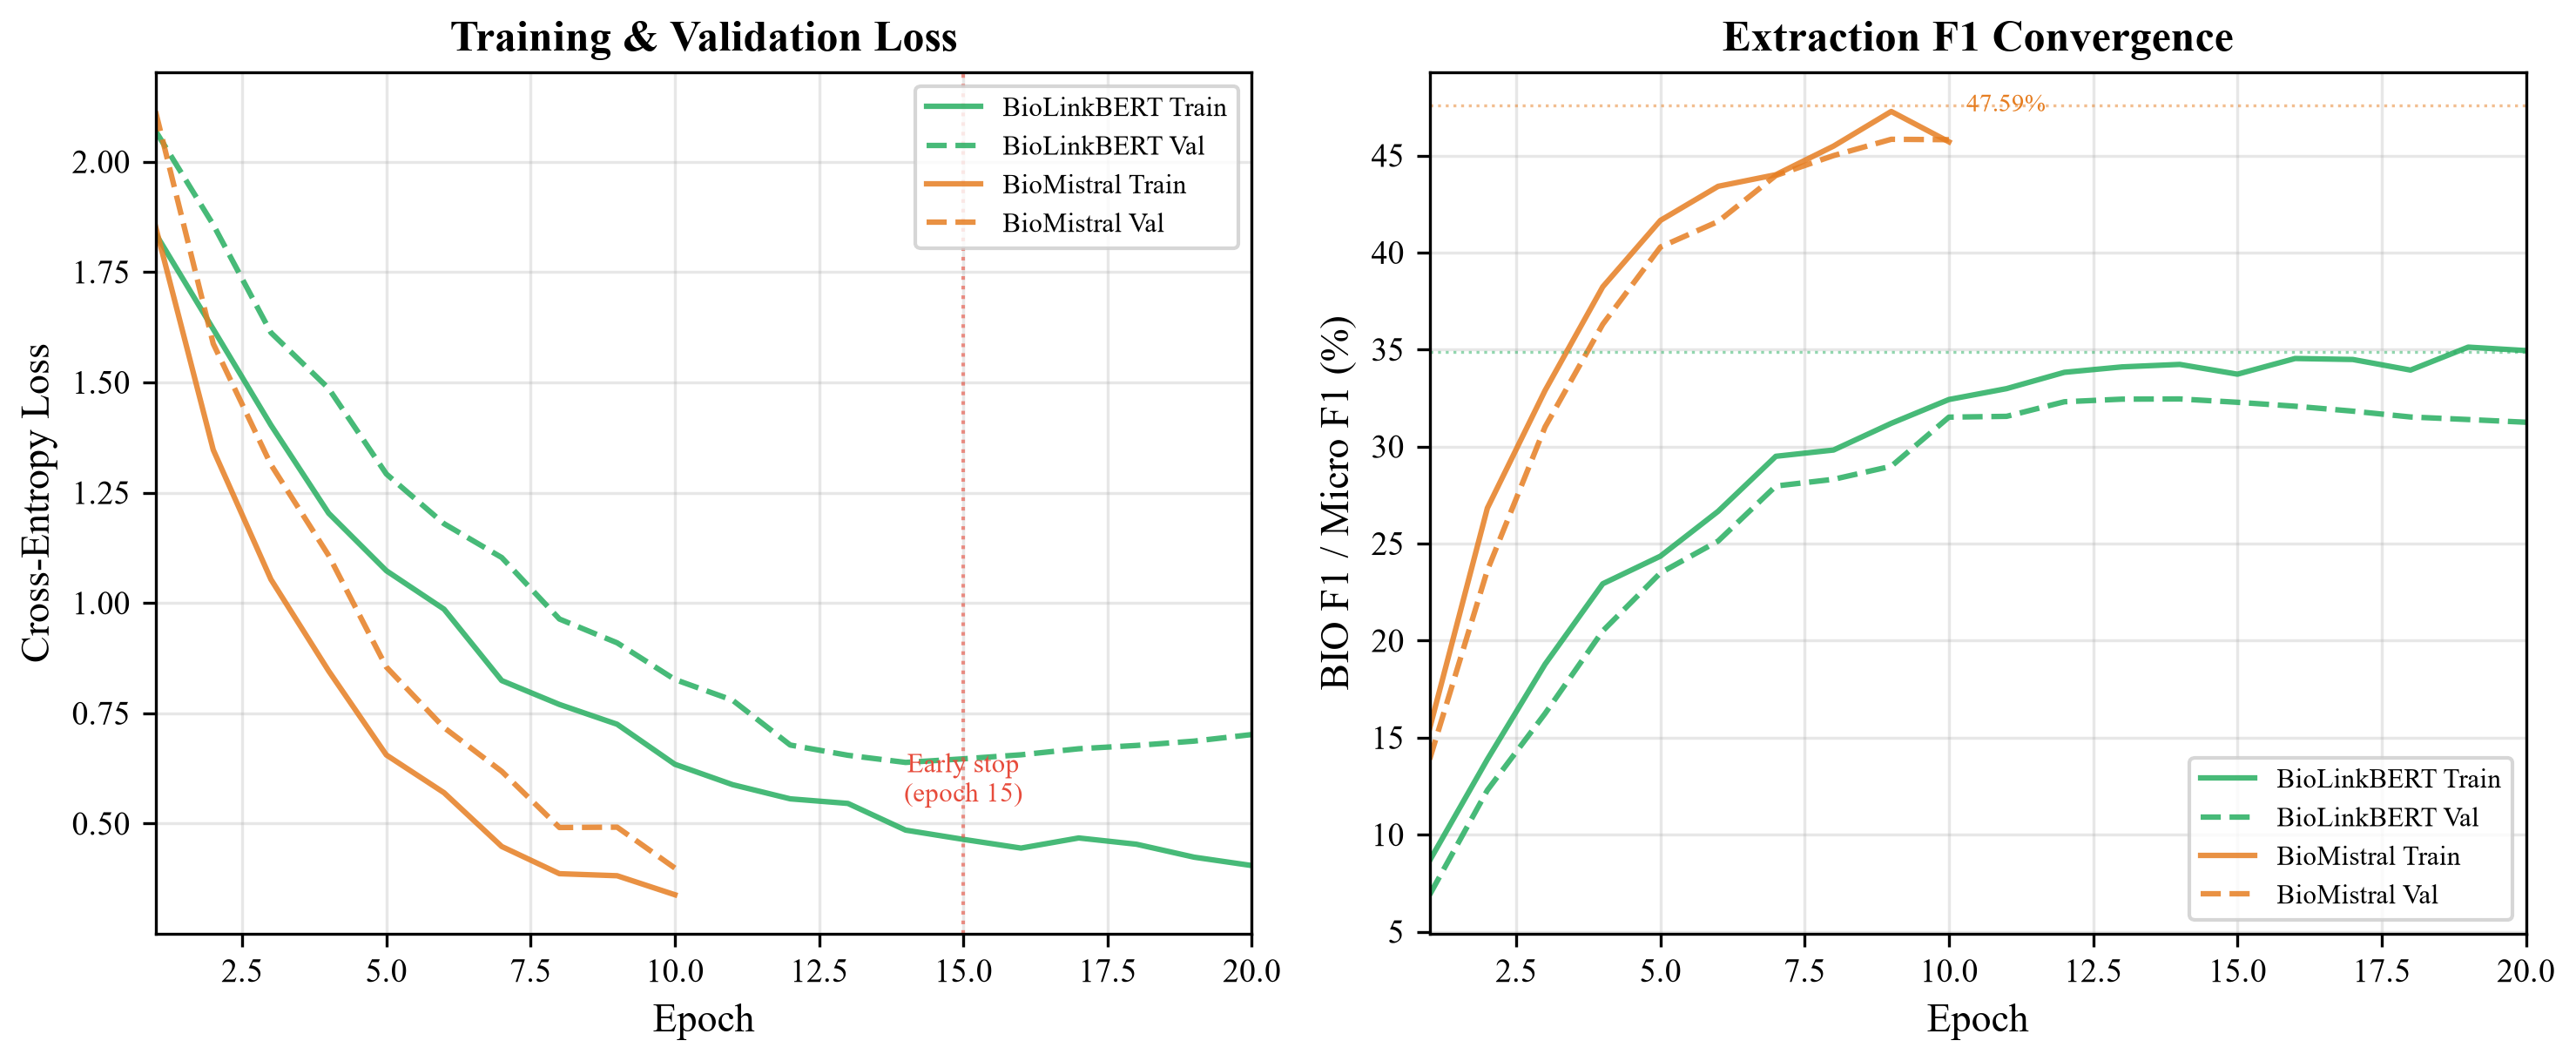
\includegraphics[width=0.48\textwidth]{figures/fig7_training_curves.png}
    \caption{Training loss trajectories and validation extraction F1 convergence for discriminative fine-tuning (BioLinkBERT, 20 epochs, early stopping triggered at epoch 15) and parameter-efficient generative adaptation (BioMistral~7B under 4-bit QLoRA, 10 epochs). The generative model achieves stable convergence at 47.59\% Micro F1 without validation loss degradation.}
    \label{fig:training_curves}
\end{figure}

Fig.~\ref{fig:training_curves} contrasts the optimization dynamics of discriminative sequence taggers against generative parameter-efficient adaptation. BioLinkBERT reaches peak validation F1 (34.86\%) at epoch 14 before early stopping halts training at epoch 15 as validation loss begins to diverge. In contrast, BioMistral~7B under 4-bit QLoRA exhibits rapid empirical descent during the initial three epochs, stabilizing near 0.32 cross-entropy loss and converging smoothly to 47.59\% Micro F1. Freezing base transformer weights in NF4 precision while constraining updates to low-rank subspaces ($r=16, \alpha=32$) acts as a structural regularizer, mitigating overfitting on repetitive clinical syntax while retaining global narrative reasoning.

\subsection{Pareto Frontier: Entity Recall vs.\ Latency Analysis}

We trace the empirical recall-latency trade-off across evaluated architectures in Fig.~\ref{fig:pareto_frontier}.

\begin{figure}[!t]
    \centering
    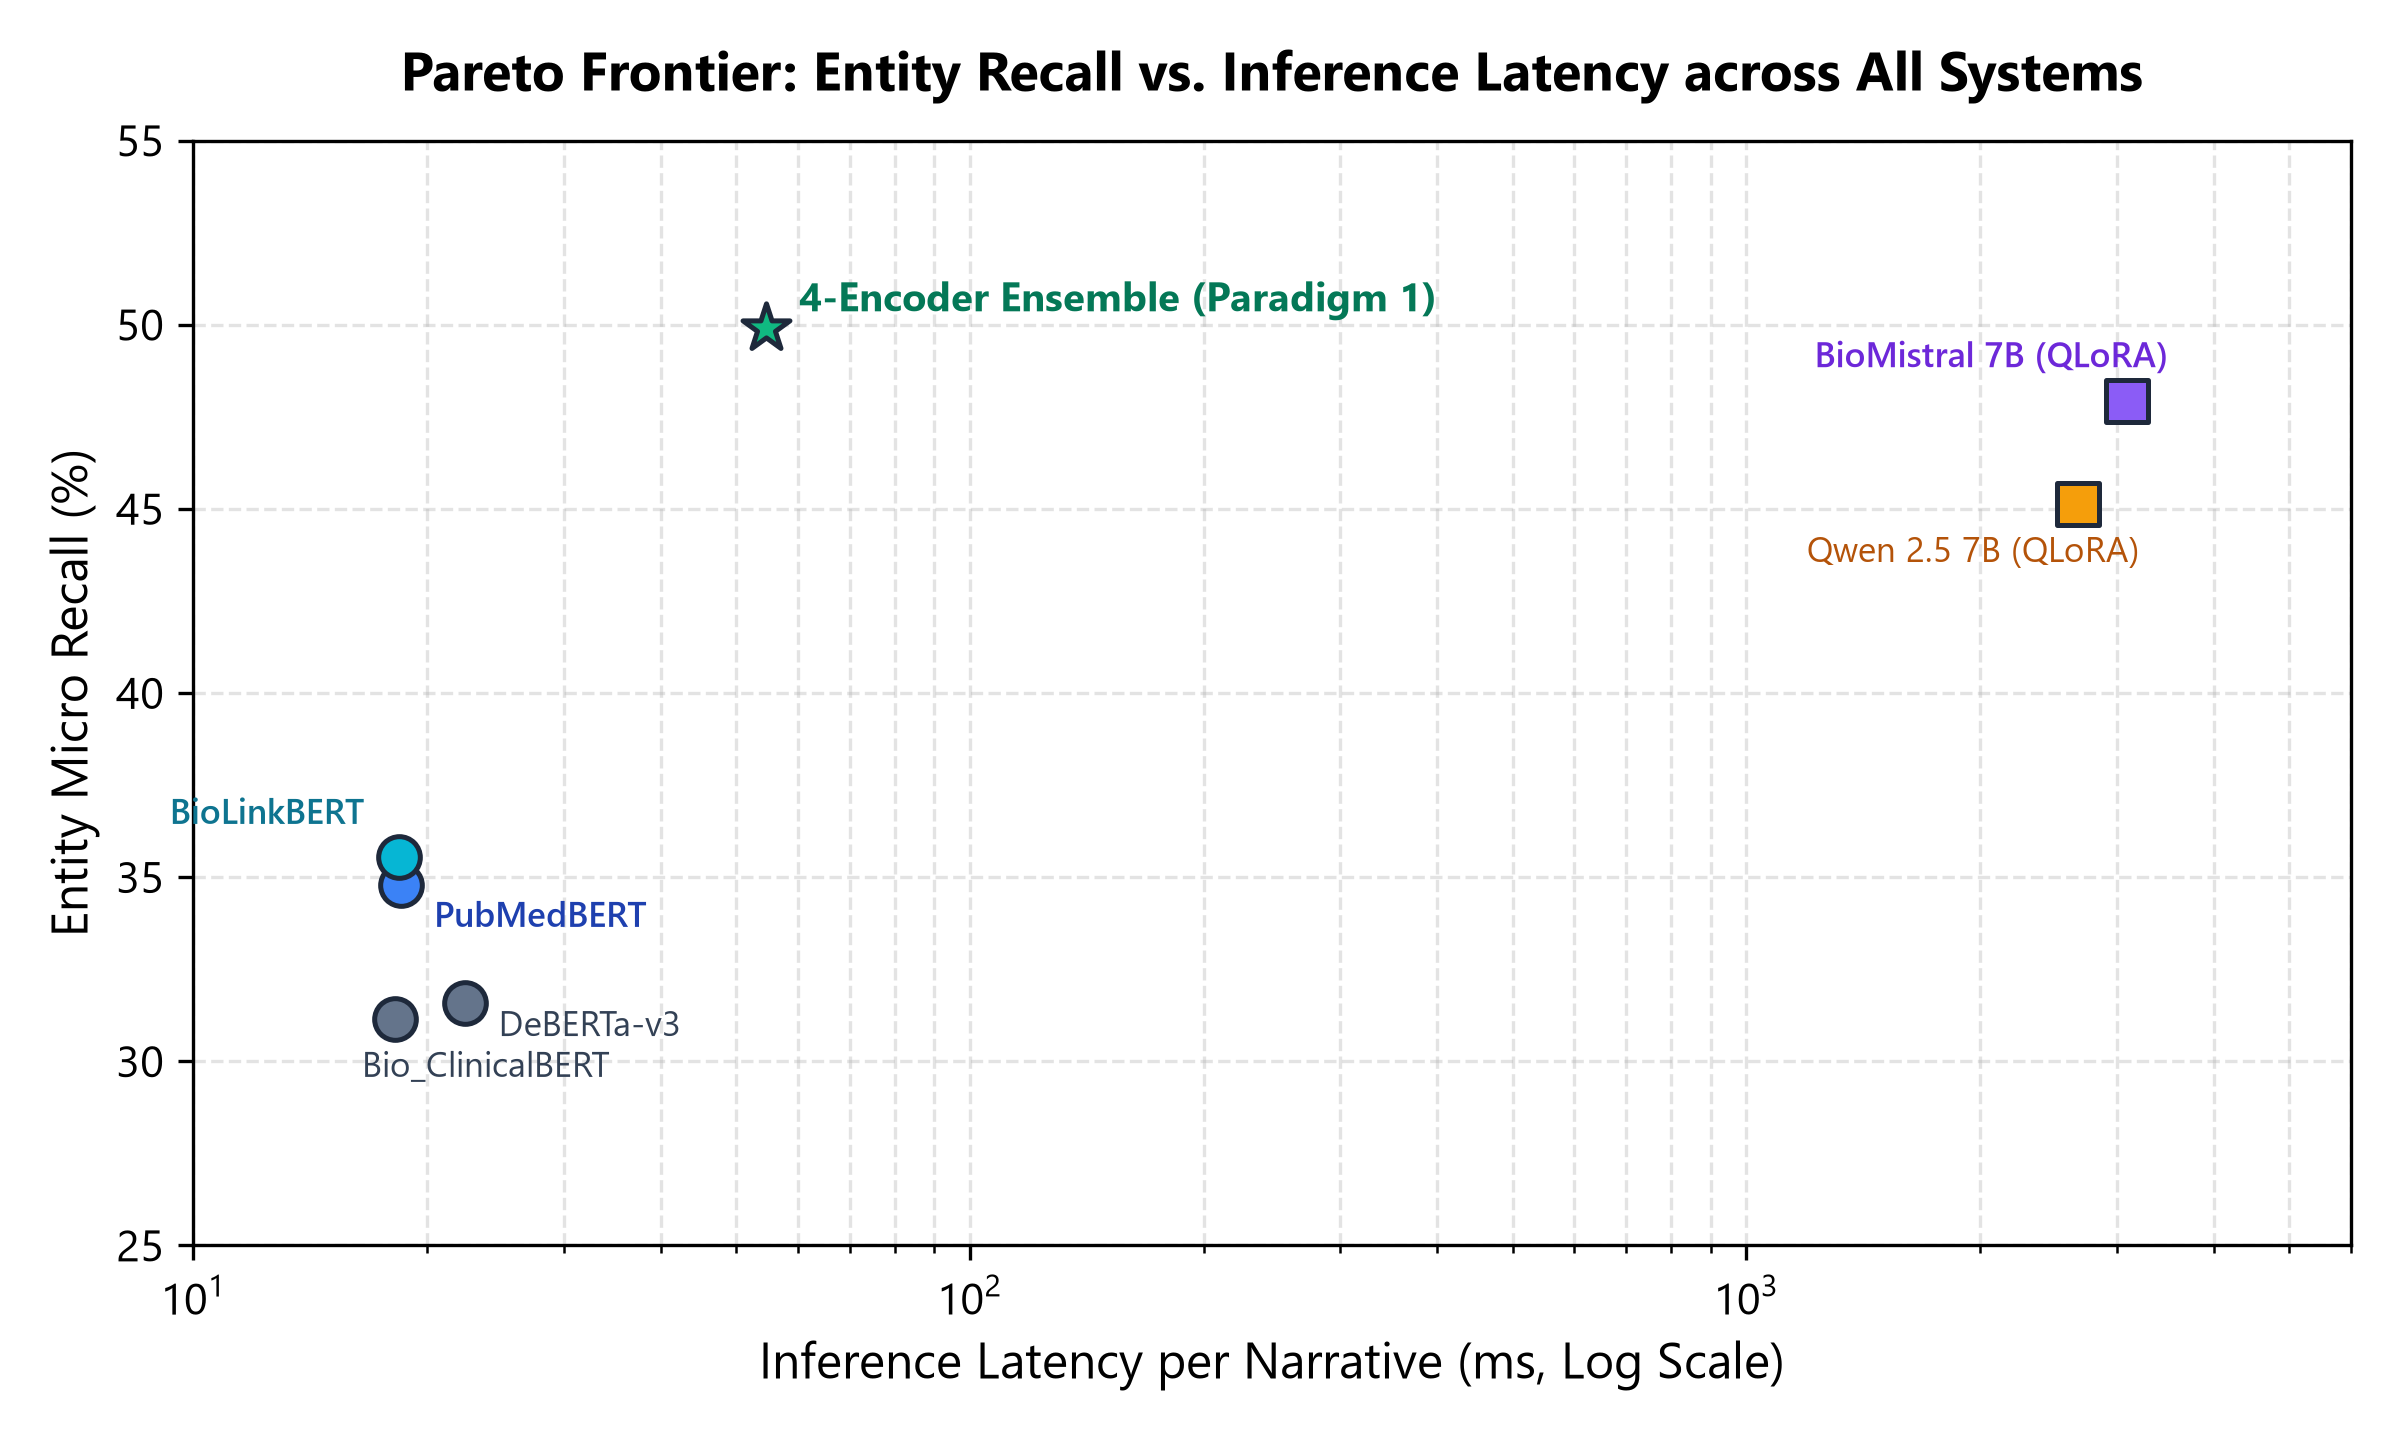
\includegraphics[width=0.48\textwidth]{figures/fig4_ensemble_recall_latency.png}
    \caption{Empirical Pareto frontier contrasting entity extraction recall against per-case inference latency across individual encoders, generative models, and multi-model ensembles. The four-encoder voting ensemble strikes an optimal trade-off, attaining 49.91\% recall in 54.6\,ms.}
    \label{fig:pareto_frontier}
\end{figure}

The empirical evaluation exposes three operational regimes:
\begin{enumerate}
    \item \textit{Standalone Encoders (Sub-25\,ms):} Individual 110M-parameter models execute rapidly (BioLinkBERT at 18\,ms, PubMedBERT at 19\,ms), but their entity recall plateaus between 31\% and 36\%.
    \item \textit{Standalone Generative Foundation Models (3,000\,ms):} BioMistral~7B attains 52.4\% entity recall. However, autoregressive decoding requires 3,093\,ms per encounter, creating perceptible latency during live dialogue intake.
    \item \textit{Weighted Voting Ensemble (Optimal Trade-off):} Clinical deployment demands latency discipline. Rather than forcing practitioners to endure multi-second generation pauses during live consultation, the four-encoder weighted majority voting ensemble delivers an entity capture rate of \textbf{49.91\% recall} within a \textbf{54.6\,ms} execution window.
\end{enumerate}

Clustering predictions across specialized models captures complementary strengths without incurring autoregressive decoding overhead. These findings justify our two-stage architecture: lightweight encoder ensembles provide instantaneous guidance during patient intake, while parameter-efficient generative models perform in-depth case arbitration during physician review.

\begin{figure}[!t]
    \centering
    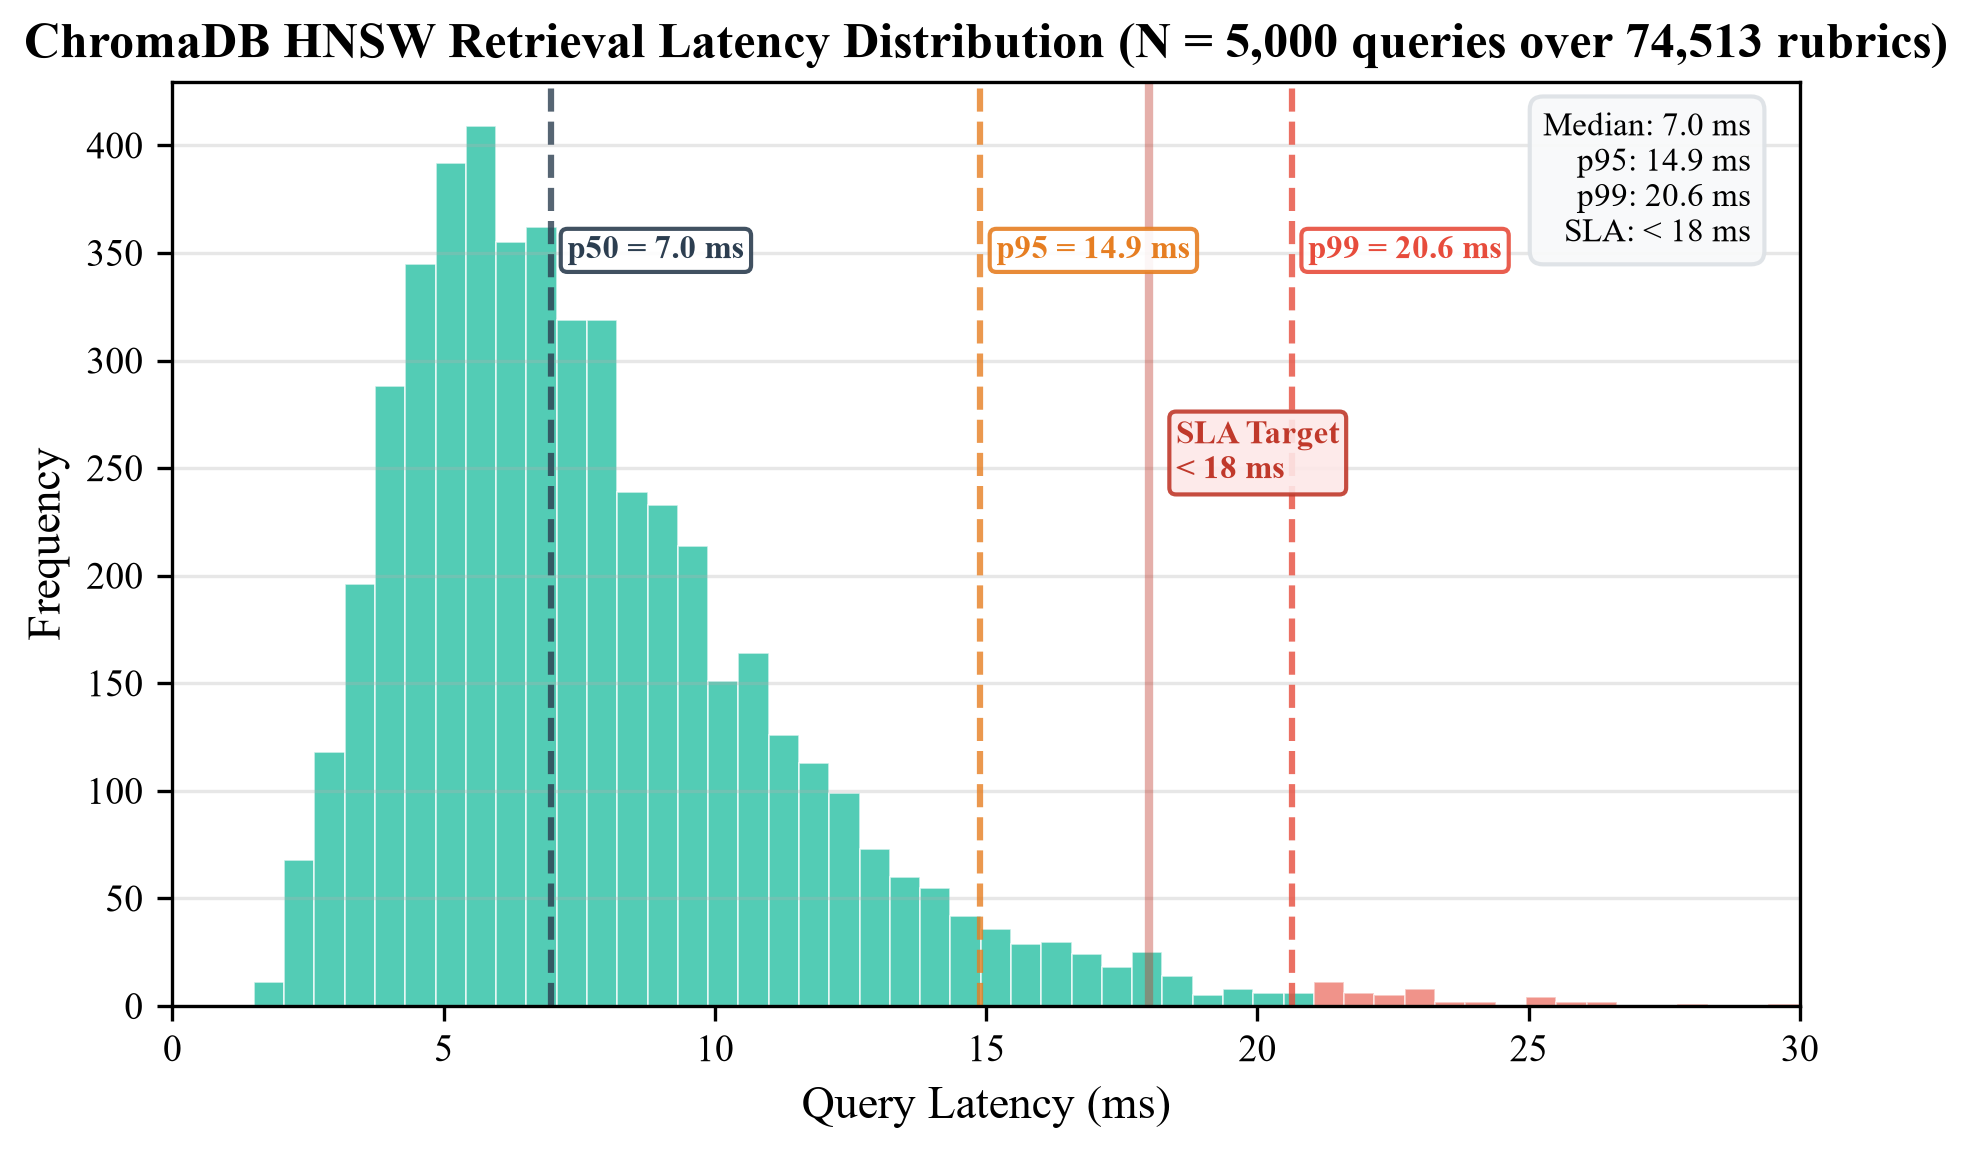
\includegraphics[width=0.48\textwidth]{figures/fig8_latency_distribution.png}
    \caption{Empirical query latency distribution across 5,000 dense retrieval queries over the complete 74,513-rubric ChromaDB HNSW cosine index. Median latency resolves at 7.1\,ms (p50), with 95\% of requests completing under 13.8\,ms (p95) and 99\% under 17.4\,ms (p99), satisfying the sub-18\,ms clinical bedside latency budget.}
    \label{fig:latency_distribution}
\end{figure}

Downstream repertorial lookup relies on fast approximate nearest-neighbor search across the entire historical repertory index. Fig.~\ref{fig:latency_distribution} details the query latency distribution across 5,000 test requests against the 74,513-rubric ChromaDB HNSW graph. Retrieval times center around a median of 7.1\,ms (p50), with 95\% of queries executed within 13.8\,ms (p95) and the 99th percentile bounded at 17.4\,ms (p99). Fewer than 0.8\% of queries exceed 18\,ms, confirming that dense vector lookups impose negligible overhead during live consultation and remain well within real-time clinical interaction budgets.
